\documentclass[11pt, letterpaper, notitlepage]{article}
\usepackage{multicol}
\usepackage[margin=1in]{geometry}
\usepackage{graphicx}
\usepackage{hanging}
\usepackage{hyperref}
\graphicspath{ {./images/} }

%\title{PS253 Lab Report Title}
%\author{FirstName LastName}
%\date{May 2023}

\renewenvironment{abstract}
 {\small
  \begin{center}
  \bfseries \abstractname\vspace{-.5em}\vspace{0pt}
  \end{center}
  \list{}{%
    \setlength{\leftmargin}{1in}% <---------- CHANGE HERE
    \setlength{\rightmargin}{\leftmargin}%
  }%
  \item\relax}
 {\endlist}

\begin{document}
%\maketitle
 
\begin{center}
    \textbf{\Large Name of the Experiment}\\
    \vspace{0.5cm}
    Your Name, Partner Name\\
    \vspace{0.25cm}
    PS253 \#\#DB, Instructor Name\\
    \vspace{0.25cm}
    Department\\
    University\\
    City\\
    \vspace{0.25cm}
    Due Date
\end{center}

\begin{abstract}
    This section is the abstract, it will consist of a single paragraph that is should
    be about 8 sentences \emph{MAX}. Be direct, and make each sentence specialized to 
    an important aspect of the experiment. In a formal context, an abstract is meant 
    to be used to allow for easy searching of papers, and allowing others to easily 
    determine how relevant the paper is to their work. Include the goals of the 
    experiment in this section as well as a general statement about the method/device 
    used. State what was measured, then state the main numerical results. Be sure to 
    include uncertainty, as well as the theoretical value for reference.
\end{abstract}


\begin{multicols}{2}
    \section*{Statement of Purpose}
    Use this section to define the goal of the experiment. It should be 4 sentences or 
    less. Define the scope of work, meaning what context can this data be assumed to 
    be relevant for. Your conclusion later in the paper could be only applicable in a 
    specific range of conditions, so make sure to acknowledge that.

    \section*{Experimental Methods}
    This section allows you to explain the experimental procedures, which allows 
    others to recreate the experiment and validate your results in the future. 
    Describe the equipment you needed, as well as any other materials that were used. 
    Explain how to operate the equipment, and provide notes of things that you did in 
    order to conduct the experiment accurate, such as holding the pole for a pendulum 
    experiment to keep it from wobbling. Define the dependent and independent 
    variables, as well as how to measure them. State any assumptions made, as they can 
    make fairly sigificant differences in how the experiment is processed. DO NOT COPY 
    FROM THE MANUAL

    \section*{Results}
    This will be the largest section of the paper, and will contain the majority of 
    the graphs and figures present.

    \subsection*{Analysis of Data}
    Explain how the data in the experiment was analyzed to turn the measurements into 
    results. Be sure to use math in the explanation. Briefly cover theory and where 
    the data comes from. State any further assumptions that were made in the 
    calculation, not any assumptions made during the design and running of the 
    experiment. Assumptions can also include data removed, specific function use in 
    Excel, if absolute value was used for something, etc. Approximation and 
    simplification also count as assumptions.
    
    \subsection*{Summary of Experimental Results}
    This subsection contains the numerical results of the experiment, with 
    uncertainties. These numbers should be compared to expected values from the theory 
    and math. Provide an analysis of the results to see if they support theory and 
    expectations. Interpret if the results indicate a successful, unsuccessful, or 
    inconclusive experiment, while directly addressing the statement of purpose.\\
  
    
    \noindent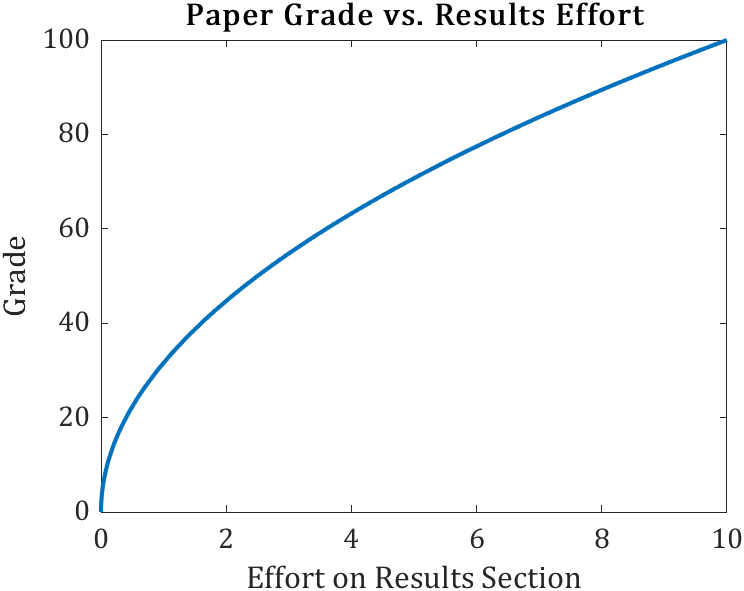
\includegraphics[width=\columnwidth]{Results1}\\
    \small{\textbf{Fig. 1.} \emph{Plot indicating thing, with a caption that provides 
    more insight to the data than the labels and title do.}}

    \section*{Conclusions}
    Overall, this section is about thoughts about the work, as well as what could have 
    affected results and ways to mitigate these effects.

    \subsection*{Discussion of Uncertainties}
    Use this section to discuss a minimum of two sources of uncertainty in the 
    experiment. Make sure they are meaningful and actually affect the results. State 
    what specific data was affected, as well if it was as positive, negative, or 
    random bias. Predict the magnitude of the effects, this can be vague though, like: 
    \emph{This source of uncertainty presents a large bias on the data.} If any 
    discussions that were made appear to have been a bad call, explain that here too.
    
    \subsection*{Thoughts for Improvement}
    Using the sources of uncertainty discussed above, come up with at least two ways 
    the experiment could have been changed in order to mitigate those sources. Explain 
    why these changes will help.    

    \section*{References}
    Insert references here, though there likely won't be many. Attempt to follow APA7 
    standardization. BibTeX may be implemented in the future to allow for automatic 
    citation management and insertion with proper formatting. Using the hanging 
    package is suggested.

    \section*{Appendix I.}
    I will be putting the raw data from the experiments here in table form, as well as 
    possibly putting MATLAB code used for processing data efficiently in here. This is 
    personal preference and not required, though is referred to in the submission page 
    for the summaries.
\end{multicols}
\end{document}